\documentclass{article}
\usepackage[a4paper,margin=2cm]{geometry}

\usepackage{graphicx}
\usepackage{xcolor}
\usepackage{subcaption}

\usepackage[utf8]{inputenc}
\usepackage[polish]{babel}
\usepackage{polski}
\usepackage[T1]{fontenc}

\usepackage{listings}
\lstdefinestyle{csharp}{
    language=[Sharp]C,
    basicstyle=\ttfamily\scriptsize,
    keywordstyle=\color{blue},
    stringstyle=\color{red},
    commentstyle=\color{green!50!black},
    numbers=left,
    numberstyle=\tiny,
    numbersep=3pt,
    breaklines=true,
    showstringspaces=false,
    frame=single,
    tabsize=4,
}

\lstset{
  language=[Sharp]C,
  basicstyle=\ttfamily\small,
  breaklines=true,
  literate=
    {ą}{{\k{a}}}1
    {Ą}{{\k{A}}}1
    {ć}{{\'{c}}}1
    {Ć}{{\'{C}}}1
    {ę}{{\k{e}}}1
    {Ę}{{\k{E}}}1
    {ł}{{\l{}}}1      % or {\l}
    {Ł}{{\L{}}}1
    {ń}{{\'{n}}}1
    {Ń}{{\'{N}}}1
    {ó}{{\'{o}}}1
    {Ó}{{\'{O}}}1
    {ś}{{\'{s}}}1
    {Ś}{{\'{S}}}1
    {ź}{{\'{z}}}1
    {Ź}{{\'{Z}}}1
    {ż}{{\.{z}}}1
    {Ż}{{\.{Z}}}1,
}

\title{Organizacja Systemów Komputerowych - Laboratorium 1.}
\author{Bartosz Zwoliński 198017, Jan Wiśniewski 197582}

\begin{document}
\maketitle

\section{Opis realizowanego zadania}
Opracowano kalkulator wyposażony w zegar. Aplikacja umożliwia rozwiązywanie równań wprowadzanych za pomocą przycisków dostępnych w oknie programu. Zaimplementowano dwa tryby wyświetlania zegara: analogowy oraz cyfrowy.

Program został zrealizowany w technologii Windows Forms z wykorzystaniem języka C\#. Aplikacja działa wyłącznie na komputerach z systemem operacyjnym Windows.

\begin{figure}[h]
    \centering
    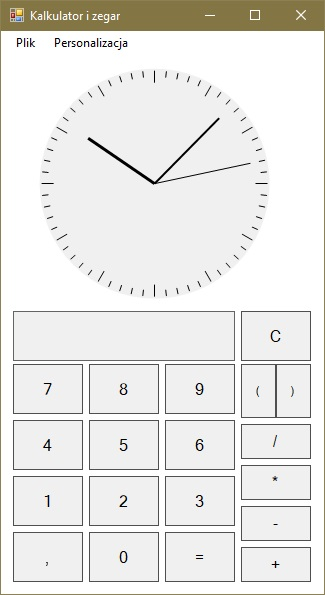
\includegraphics[width=0.3\linewidth]{default_look.jpg}
    \caption{Domyślny wygląd programu}
\end{figure}

\section{Metody implementacji}
\subsection{Kalkulator}
Obliczanie równania wprowadzonego do kalkulatora realizowane jest poprzez przekształcenie zapisu infiksowego do odwrotnej notacji polskiej, a następnie wykonanie obliczeń dla tak przygotowanego wyrażenia. Zastosowano takie rozwiązanie, aby umożliwić obsługę równań zawierających wiele operatorów.

\begin{figure}
\begin{lstlisting}[style=csharp]
private List<string> Convert_To_RPN(object sender, EventArgs e)
{
    Label label = sender as Label;
    Stack<char> stack = new Stack<char>();
    string expression = label.Text;
    List<string> output = new List<string>();
    StringBuilder number = new StringBuilder();

    for (int i = 0; i < expression.Length; i++)
    {
        char c = expression[i];

        if (char.IsDigit(c) || c == ',' || (c == '-'  & number.Length == 0)) number.Append(c);
        else
        {
            if (number.Length > 0)
            {
                output.Add(number.ToString());
                number.Clear();
            }

            if (c == '+' || c == '-' || c == '*' || c == '/')
            {
                while (stack.Count > 0 && stack.Peek() != '(' && GetPrecedence(stack.Peek()) >= GetPrecedence(c))
                {
                    output.Add(stack.Pop().ToString());
                }
                stack.Push(c);
            }
            else if (c == '(') stack.Push(c);
            else if (c == ')')
            {
                try
                {
                    while (stack.Count > 0 && stack.Peek() != '(')
                    {
                        output.Add(stack.Pop().ToString());
                    }

                    stack.Pop();
                }
                catch
                {
                    this.valid_RPN = false;
                    return null;
                }
            }
            else if (c != ' ')
            {
                this.valid_RPN = false;
                return null;
            }
        }
    }

    if (number.Length > 0) output.Add(number.ToString());
    
    while (stack.Count > 0)
    {
        if (stack.Peek() == '(')
        {
            this.valid_RPN = false;
            return null;
        }
        output.Add(stack.Pop().ToString());
    }

    this.valid_RPN = true;
    return output;
}
private int GetPrecedence(char op)
{
    switch (op)
    {
        case '+':
        case '-':
            return 1;
        case '*':
        case '/':
            return 2;
        default:
            return 0;
    }
}
\end{lstlisting}
\caption{Realizacja konwersji z zapisu infiksowego do odwrotnej notacji polskiej (ONP)}
\end{figure}

Algorytm konwersji zapisu równania polega na umieszczaniu operatorów na stosie, skąd są one następnie zdejmowane zgodnie z kolejnością wykonywania działań oraz występowaniem liczb w równaniu. Tak przetworzone wyrażenie jest następnie obliczane, a wynik wyświetlany w oknie, w którym wprowadzono równanie.

\begin{figure}
\begin{lstlisting}[style=csharp]
private float Solve_RPN(List<string> rpn)
{
    float result = 0;
    Stack<float> stack = new Stack<float>();
    string number = null;
    if (rpn == null) return 0;
    for (int i = 0; i < rpn.Count; i++)
    {
        string element = rpn[i];
        if (float.TryParse(element,out _))
        {
            number = element;
        }
        if (!string.IsNullOrEmpty(number))
        {
            stack.Push(float.Parse(number.Replace(',','.')));
            number = null;
        }
        if ((element == "+" || element == "-" || element == "*" || element == "/") & stack.Count > 0)
        {
            float a = stack.Pop();
            float b = stack.Pop();
            switch (element)
            {
                case "+":
                    result = b + a;
                    break;
                case "-":
                    result = b - a;
                    break;
                case "*":
                    result = b * a;
                    break;
                case "/":
                    result = b / a;
                    break;
            }
            stack.Push(result);
        }
        
    }
    if (stack.Count > 0) return stack.Pop();
    else return float.Parse(number);
}
\end{lstlisting}
\caption{Realizacja rozwiązania równania w postaci ONP}
\end{figure}
\subsection{Interfejs}
Wprowadzanie danych do kalkulatora odbywa się za pomocą przycisków umieszczonych pod zegarem. Dostępne są przyciski umożliwiające wprowadzanie cyfr, przecinka oraz operatorów dodawania, odejmowania, mnożenia, dzielenia i nawiasów. Zaimplementowano również przycisk \emph{C}, który usuwa zawartość pola wejściowego.

Dodatkowo program obsługuje wprowadzanie danych z klawiatury. Oprócz działania odpowiadającego przyciskom widocznym na ekranie, klawisz Enter pełni funkcję znaku „=”, natomiast klawisz Backspace umożliwia usuwanie znaków pojedynczo z pola wejściowego.

\subsection{Zegary}
Zegar analogowy posiada trzy wskazówki wskazujące aktualną godzinę, minutę oraz sekundę, a także znaczniki ułatwiające odczyt czasu. Jest on rysowany na podstawie kąta obrotu poszczególnych wskazówek, wyznaczanego dla bieżącej chwili.

Zegar cyfrowy składa się z czterech siedmiosegmentowych wyświetlaczy prezentujących godzinę i minutę. Każdy segment może znajdować się w jednym z dwóch stanów: włączonym lub wyłączonym. Na podstawie aktualnego czasu aktywowane są odpowiednie segmenty zgodnie z zapisanymi kombinacjami. Pomiędzy wyświetlaczami znajduje się dwukropek, który pulsuje co sekundę.

Aktualny czas odczytywany jest z wykorzystaniem obiektu \emph{Timer}.

\begin{figure}
    \centering
    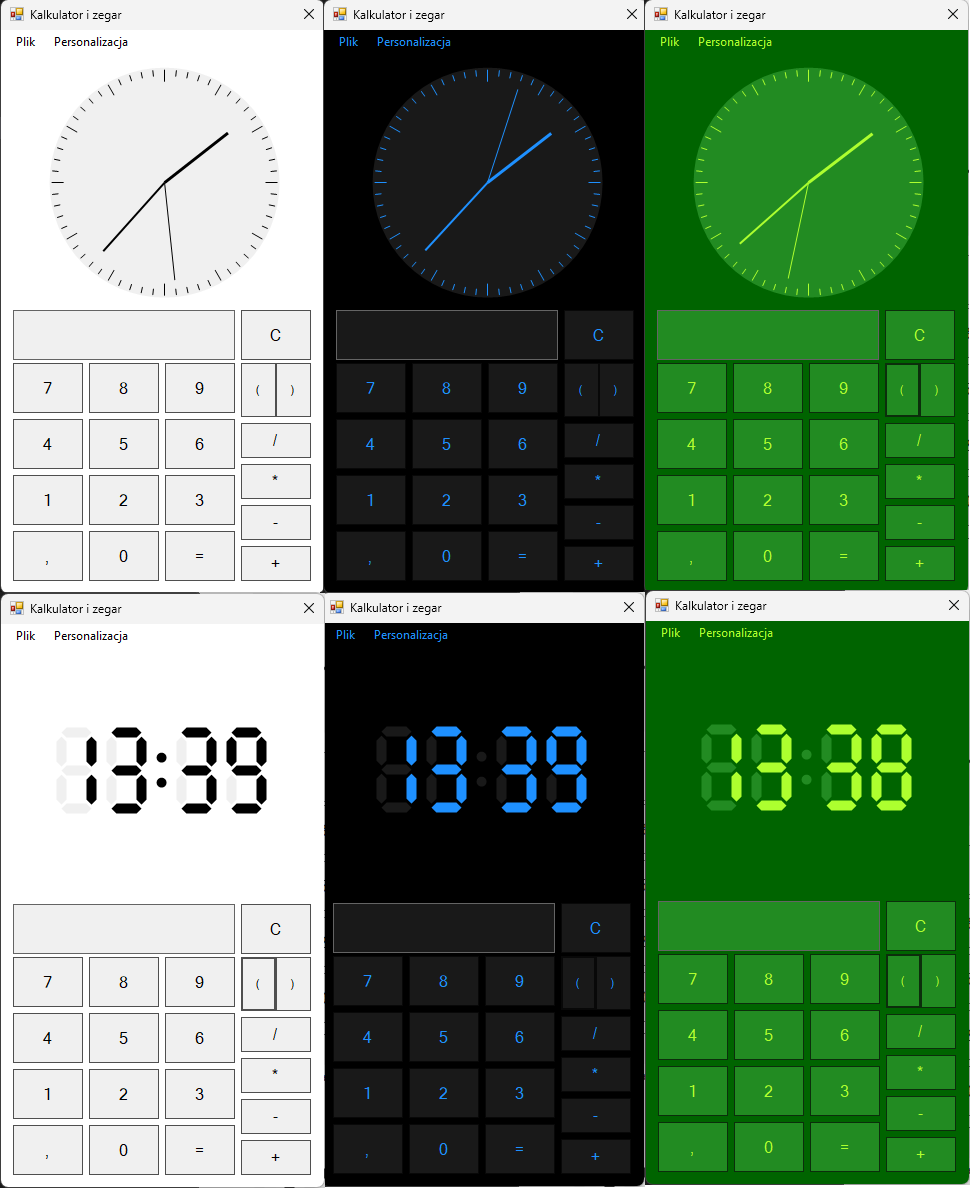
\includegraphics[width=0.4\linewidth]{zestawienie_personalizacji.png}
    \caption{Zestawienie wszystkich dostępnych motywów i zegarów}
\end{figure}

W celu umożliwienia użytkownikowi zmiany wyglądu programu oraz typu zegara zaimplementowano menu, w którym znajdują się odpowiednie opcje. Zaimplementowano motywy: domyślny, ciemny i zielony oraz wcześniej opisane style zegarów analogowy i cyfrowy.


\begin{figure}
    \centering
    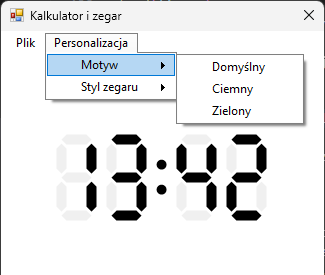
\includegraphics[width=0.4\linewidth]{menu.png}
    \caption{Menu wyboru motywu}
\end{figure}

\section{Podsumowanie i potencjalne poprawki}
Program realizuje założone funkcje. Zastosowana metoda implementacji kolorystyki okna umożliwia łatwe dodawanie kolejnych stylów, co zwiększa możliwości personalizacji interfejsu przez użytkownika.

Do głównych ograniczeń programu należy brak obsługi niektórych operatorów matematycznych, takich jak pierwiastek, logarytm czy potęga. Ulepszenie aplikacji mogłoby również polegać na dodaniu kursora do pola wprowadzania danych, co pozwoliłoby na swobodniejszą edycję równania w dowolnym miejscu.

\end{document}